% Set a pdf version and a document type
\ifx\pdfminorversion\undefined\else\pdfminorversion=4\fi
\documentclass[aspectratio=169,t,table]{beamer}

% Import all necessary packages
% Use this file to import all packages which are needed for the lecture
\usepackage[english]{babel}
\usepackage[utf8]{inputenc}
\usepackage[sfdefault]{roboto}
\usepackage[T1]{fontenc}
\usepackage{amsmath,amssymb}
\usepackage{graphicx}
\usepackage{listings}
\usepackage[backend=biber,sorting=none,doi=true,style=ieee]{biblatex}
\usepackage{url}
\usepackage{hyperref}
\usepackage{fontawesome5}
\usepackage{graphicx}
\usepackage{booktabs}
\usepackage{calc}
\usepackage{ifthen}
\usepackage{tabularx}
\usepackage{longtable}
\usepackage{makecell}
\usepackage{multicol}
\usepackage{multirow}
\usepackage{hhline}
\usepackage{qrcode}
\usepackage{xcolor}
\usepackage{cleveref}
\usepackage{tikz}
\usepackage{tikz-cd}
\usepackage{pgfplots,pgfplotstable,pgf-pie}
\usepackage[linesnumbered]{algorithm2e}
\usepackage{array}
\usepackage{mathtools}
\usetikzlibrary{patterns}
\usetikzlibrary{arrows.meta}


% Set the theme (customized FAU beamer theme)
\usetheme[%
	image,%
	longtitle,%
	inst=tf%
]{fau}

% Set all important settings and define commands that are used in more than one lecture
% English version FAU Logo
\usepackage[english]{babel}
% German version FAU Logo
%\usepackage[ngerman]{babel}

\usepackage[utf8]{inputenc}
\usepackage[T1]{fontenc}
\usepackage{amsmath,amssymb}
\usepackage{graphicx}
\usepackage{listings}
\usepackage[backend=biber,sorting=none,doi=true,style=ieee]{biblatex}

% Options:
%  - inst:      Institute
%                 med:      MedFak FAU theme
%                 nat:      NatFak FAU theme
%                 phil:     PhilFak FAU theme
%                 rw:       RWFak FAU theme
%                 rw-jura:  RWFak FB Jura FAU theme
%                 rw-wiso:  RWFak FB WISO FAU theme
%                 tf:       TechFak FAU theme
%  - image:     Cover image on title page
%  - plain:     Plain title page
%  - longtitle: Title page layout for long title
\usetheme[%
	image,%
	longtitle,%
	inst=tf%
]{fau}

% Enable semi-transparent animation preview
\setbeamercovered{transparent}

% Enable frame numbering
%\setbeamertemplate{footline}[frame number]


\lstset{%
	language=Python,
	tabsize=2,
	basicstyle=\tt,
	keywordstyle=\color{blue},
	commentstyle=\color{green!50!black},
	stringstyle=\color{red},
	numbers=left,
	numbersep=0.5em,
	xleftmargin=1em,
	numberstyle=\tt
}

\defbibheading{bibliography}{}
\addbibresource{references.bib}

\date[SS2022]{Summer semester 2022}


\usepackage{url}
\usepackage{enumitem}
\setlist[itemize]{noitemsep, nolistsep}
\setlist[itemize]{label=\footnotesize\raisebox{.275ex}{$\bullet$}}
\usepackage{hyperref}
\usepackage{fontawesome5}
\usepackage{graphicx}
\usepackage{booktabs}
\usepackage{calc}
\usepackage{ifthen}

\usepackage{tabularx}
\usepackage{makecell}

\usepackage{xcolor}
\definecolor{airforceblue}{rgb}{0.36, 0.54, 0.66}
\definecolor{ForestGreen}{rgb}{0.34, 0.139, 0.34}

% English version
\institute[CS6]{Chair of Computer Science 6 (Data Management), Friedrich-Alexander University Erlangen-N\"urnberg}
% German version
% \institute[Lehrstuhl]{Lehrstuhl, Friedrich-Alexander-Universit\"at Erlangen-N\"urnberg}

\setbeamertemplate{section in toc}[sections numbered]

\setbeamertemplate{section page}{%
	\begingroup
	\begin{beamercolorbox}[sep=10pt,center,rounded=true,shadow=true]{section title}
		\usebeamerfont{section title}\thesection~\insertsection\par
	\end{beamercolorbox}
	\endgroup
}

\usepackage{tikz}
\usepackage{tikz-cd}
\usepackage{pgfplots,pgfplotstable,pgf-pie}

\newcommand{\tikzmark}[1]{\tikz[remember picture] \node[coordinate] (#1) {#1};}

\tikzset{
	every overlay node/.style={
			%draw=black,fill=white,rounded corners,
			anchor=north west, inner sep=0pt,
		},
}
% Usage:
% \tikzoverlay at (-1cm,-5cm) {content};
% or
% \tikzoverlay[text width=5cm] at (-1cm,-5cm) {content};
\def\tikzoverlay{%
	\tikz[remember picture, overlay]\node[every overlay node]
}%

\newcommand{\plots}{0.611201}
\newcommand{\plotm}{2.19882}

\newcommand{\MaxNumberX}{3}
\newcommand{\MaxNumberY}{5}

\pgfmathdeclarefunction{gauss}{2}{%
	\pgfmathparse{1/(#2*sqrt(2*pi))*exp(-((x-#1)^2)/(2*#2^2))}%
}

\tikzset{
	thick,
	>=latex,
	every edge/.style={draw=gray, thick, >=latex},
	vertex/.style = {
			circle,
			fill            = black,
			outer sep = 2pt,
			inner sep = 1pt,
		}
}
\usetikzlibrary{matrix,mindmap}
\usetikzlibrary{arrows,decorations.pathmorphing,backgrounds,fit,positioning,shapes.symbols,chains,intersections,snakes}
\tikzset{level 1/.append style={sibling angle=50,level distance = 165mm}}
\tikzset{level 2/.append style={sibling angle=20,level distance = 45mm}}
\tikzset{every node/.append style={scale=1}}
% read in data file
\pgfplotstableread{data/iris.dat}\iris
% get number of data points
\pgfplotstablegetrowsof{\iris}
\pgfmathsetmacro\NumRows{\pgfplotsretval-1}

\usepgfplotslibrary{groupplots}
\pgfplotsset{height=4cm,width=8cm,compat=1.14}

\tikzset{
	vertex/.style = {
			circle,
			fill            = black,
			outer sep = 2pt,
			inner sep = 1pt,
		}
}

\tikzset{
	mynode/.style={
			draw,
			thick,
			anchor=south west,
			minimum width=2cm,
			minimum height=1.3cm,
			align=center,
			inner sep=0.2cm,
			outer sep=0,
			rectangle split,
			rectangle split parts=2,
			rectangle split draw splits=false},
	reverseclip/.style={
			insert path={(current page.north east) --
					(current page.south east) --
					(current page.south west) --
					(current page.north west) --
					(current page.north east)}
		}
}

\tikzset{basic/.style={
			draw,
			rectangle split,
			rectangle split parts=2,
			rectangle split part fill={blue!20,white},
			minimum width=2.5cm,
			text width=2cm,
			align=left,
			font=\itshape
		},
	Diamond/.style={ diamond,
			draw,
			shape aspect=2,
			inner sep = 2pt,
			text centered,
			fill=blue!10!white,
			font=\itshape
		}}


\tikzset{level 1/.append style={sibling angle=50,level distance = 165mm}}
\tikzset{level 2/.append style={sibling angle=20,level distance = 45mm}}
\tikzset{every node/.append style={scale=1}}

\usetikzlibrary{arrows,decorations.pathmorphing,backgrounds,fit,positioning,shapes.symbols,chains,intersections,snakes,positioning,matrix,mindmap,shapes.multipart,shapes,calc,shapes.geometric}



% Title, author(s), and date
\title[KDDmUe~2.~Introduction]{2. Introduction} %
\subtitle{Knowledge Discovery in Databases with Exercises}
\author[D.~Probst]{Dominik Probst, \texttt{dominik.probst@fau.de}}


% Metadata
\input{x-additional/vc.tex}
\hypersetup{
	pdftitle={KDDmUe - 2. Introduction},
	pdfkeywords={
		KDD, 
		KDDmUe, 
		Knowledge Discovery in Databases, 
		Knowledge Discovery in Databases with Exercises, 
		FAU Erlangen-Nürnberg, 
		Data Science, 
		Machine Learning, 
		Data Mining, 
		Lecture, 
		Introduction,
		Data Mining Process,
		Data Mining Challenges,
		Data Mining Applications,
		Data Mining Interdisciplinary Context,
		Version \GITAbrHash
	},
	pdfsubject={Introductory lecture on data mining/KDD: its purpose, process, challenges, applications, and interdisciplinary context.},
	pdfcreator={Dominik Probst, CS6, FAU Erlangen-Nürnberg},
	pdflang={English}
}

% Start the document
\begin{document}

% Title
\maketitle

{ % Outline
	\setbeamertemplate{footline}{}
	\begin{frame}[noframenumbering]{Outline}
		\tableofcontents

	\end{frame}
}

% Body
\section{Why data mining?}

\begin{frame}{Why Data Mining? (I)}
	\textbf{The explosive growth of data: from terabytes to petabytes and
		more.}\\
	\begin{itemize}
		\item Data collection and availability:
		      \begin{itemize}
			      \item Automated data collection tools.
			      \item Database systems.
			      \item World wide web.
			      \item Computerized society.
			      \item Digitization.
		      \end{itemize}
		\item Major sources of abundant data:
		      \begin{itemize}
			      \item Business: web, e-commerce, transactions, stocks \ldots
			      \item Science: remote sensing, bioinformatics, scientific
			            simulation \ldots
			      \item Society: news, digital cameras, social media \ldots
		      \end{itemize}
		\item The era of \textbf{big data} (as inflationary used buzzword).
	\end{itemize}
\end{frame}

\begin{frame}{Why Data Mining? (II)}
	\textbf{The initial situation:}
	\begin{itemize}
		\item We are drowning in  data
		\item We are starving for knowledge
	\end{itemize}
	\textbf{The basic idea behind data mining:}
	\begin{itemize}
		\item We can analyze the data to satisfy our hunger for knowledge
	\end{itemize}
\end{frame}

\begin{frame}{Evolution of Sciences (I)}
	\begin{itemize}
		\item Before $1600$, era of \textbf{empirical science}.
		\item $1600-1950$s, rise of \textbf{theoretical science}.
		      \begin{itemize}
			      \item Each discipline has grown a theoretical component.
			      \item Theoretical models often motivate experiments and generalize
			            our understanding.
		      \end{itemize}
		\item $1950-1990$s, rise of \textbf{computational science}.
		      \begin{itemize}
			      \item Over the last $50$ years most disciplines have grown a third,
			            computational branch.
			            \begin{itemize}
				            \item E.g. empirical, theoretical, and computational ecology.
				            \item E.g. physics, linguistics or biology.
			            \end{itemize}
			      \item Computational science traditionally meant simulation.
			      \item It grew out of our inability to describe reality by
			            closed-form mathematical models.
		      \end{itemize}
	\end{itemize}
\end{frame}

\begin{frame}{Evolution of Sciences (II)}
	\begin{itemize}
		\item $1990-$now, rise of \textbf{data science}.
		      \begin{itemize}
			      \item The flood of data from new instruments and modern simulations.
			      \item The ability to economically store and manage petabytes of
			            data.
			      \item The internet makes all these archives world wide accessible.
			      \item Scientific \emph{information management}, \\
			            acquisition,\\
			            organization, \\
			            query, and \\
			            visualization scale almost linearly with amount of data.
			      \item \textbf{Data mining} is a major new challenge!
		      \end{itemize}
		\item For further reading:\\
		      \small{Jim Gray and Alex Szaly: \emph{The World Wide Telescope: An
				      Archetype for Online Science}, \\ Communications of the ACM
			      45(11):
			      50-54, 2002.}
	\end{itemize}
\end{frame}

\begin{frame}{Evolution of Sciences (III)}
	\begin{itemize}
		\item $1960$s: Data collection, database creation, \\
		      \hspace{1cm} integrated management systems (IMS), and \\
		      \hspace{1cm} network database management systems (DBMS).
		\item $1970$s: Relational data model, relational DBMS implementation
		      (RDBMS).
		\item $1980$s: RDBMS products, database creation, \\
		      \hspace{1cm} advanced data models (extended relational, object
		      oriented, deductive etc.),\\
		      \hspace{1cm} application-oriented DBMS (spatial, scientific,
		      engineering etc.).
		\item $1990$s: Data mining, data warehousing, multimedia databases, web
		      databases.
		\item $2000$s: Stream data management and mining,\\
		      \hspace{1cm} data mining and applications, \\
		      \hspace{1cm} web technology (XML, data integration), and global
		      information systems.
	\end{itemize}
\end{frame}

\section{What is data mining?}

\begin{frame}{What is Data Mining?}
	\textbf{Data mining or knowledge discovery from data}:
	\begin{itemize}
		\item Extraction of interesting (\textbf{non-trivial, implicit,
			      previously unknown and potentially useful}) patterns from huge amounts
		      of data.
		\item Is \textbf{data mining} a misnomer?
	\end{itemize}
	Alternative names:
	\begin{itemize}
		\item Knowledge discovery/mining in databases (KDD).
		\item Knowledge extraction.
		\item Data/pattern analysis.
		\item Data archeology/dredging.
		\item Information harvesting.
		\item Business intelligence.
	\end{itemize}
\end{frame}

\begin{frame}{Examples: Is everything Data Mining?}
	Considered to be data mining:
	\begin{itemize}
		\item Analysis of customer behavior for user-related advertising.
		\item Analysis of payment histories for fraud detection.
		\item Analysis of infection behavior for better understanding of a
		      pandemic.
	\end{itemize}
	\textbf{NOT} considered to be data mining:
	\begin{itemize}
		\item Simple search for females in a customer database.
		\item Simple join of two database tables.
		\item Simple deductive database validating a new tuple with regards to
		      predefined constraints.
	\end{itemize}
\end{frame}

\begin{frame}{Data Mining in the Database-Systems Community}
	\begin{itemize}
		\item \textbf{Knowledge discovery pipeline} is a typical view from
		      the database-systems and data-warehousing community.
		\item Data mining plays an essential role in the knowledge-discovery
		      process.
	\end{itemize}
	\vspace{0.15cm}
	\centering
	\scalebox{0.95}{%
		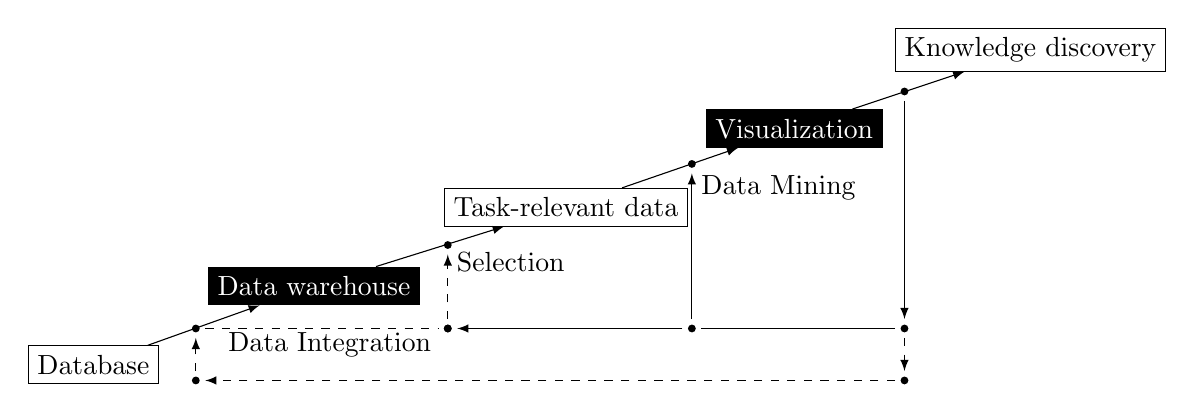
\begin{tikzpicture}
			% Dialectics
			\node[draw] (Database) at (0,0) {Database};
			\node[draw,fill=black,text=white] (Data warehouse) at (2.8,1) {Data
				warehouse};
			\node[draw] (Task-relevant data) at (6,2) {Task-relevant data};
			\node[draw,fill=black,text=white] (Data mining) at (8.9,3)
			{Visualization};
			\node[draw] (Knowledge discovery) at (11.9,4) {Knowledge discovery};

			\node (Data Integration) at (3,0.25) {Data Integration};
			\node (Selection) at (5.3,1.3) {Selection};
			\node (Data Mining) at (8.7,2.25) {Data Mining};

			\draw node[vertex] (Joint1) at (1.3,0.46) {};
			\draw node[vertex] (Joint2) at (4.5,1.52) {};

			\draw node[vertex] (Joint3) at (4.5,0.46) {};
			\draw node[vertex] (Joint7) at (4.5,0.46) {};
			\draw node[vertex] (Joint8) at (7.6,0.46) {};
			\draw node[vertex] (Joint9) at (10.3,0.46) {};
			\draw node[vertex] (Joint10) at (10.3,-0.2) {};
			\draw node[vertex] (Joint11) at (1.3,-0.2) {};

			\draw node[vertex] (Joint5) at (7.6,2.55) {};
			\draw node[vertex] (Joint6) at (10.3,3.47) {};


			\draw[->,draw=black] (Database) to (Data warehouse);
			\draw[->,draw=black] (Data warehouse) to (Task-relevant data);
			\draw[->,draw=black] (Task-relevant data) to (Data mining);
			\draw[->,draw=black] (Data mining) to (Knowledge discovery);
			\draw[-,draw=black, dashed] (Joint1) to (Joint3);
			\draw[->,draw=black, dashed] (Joint3) to (Joint2);
			\draw[->,draw=black] (Joint6) to (Joint9);
			\draw[-,draw=black] (Joint9) to (Joint8);
			\draw[->,draw=black] (Joint8) to (Joint7);
			\draw[->,draw=black] (Joint8) to (Joint5);
			\draw[->,draw=black,dashed] (Joint10) to (Joint11);
			\draw[->,draw=black,dashed] (Joint9) to (Joint10);
			\draw[->,draw=black,dashed] (Joint11) to (Joint1);
		\end{tikzpicture}
	}
\end{frame}

\begin{frame}{Data Mining in the Business Community}
	\centering
	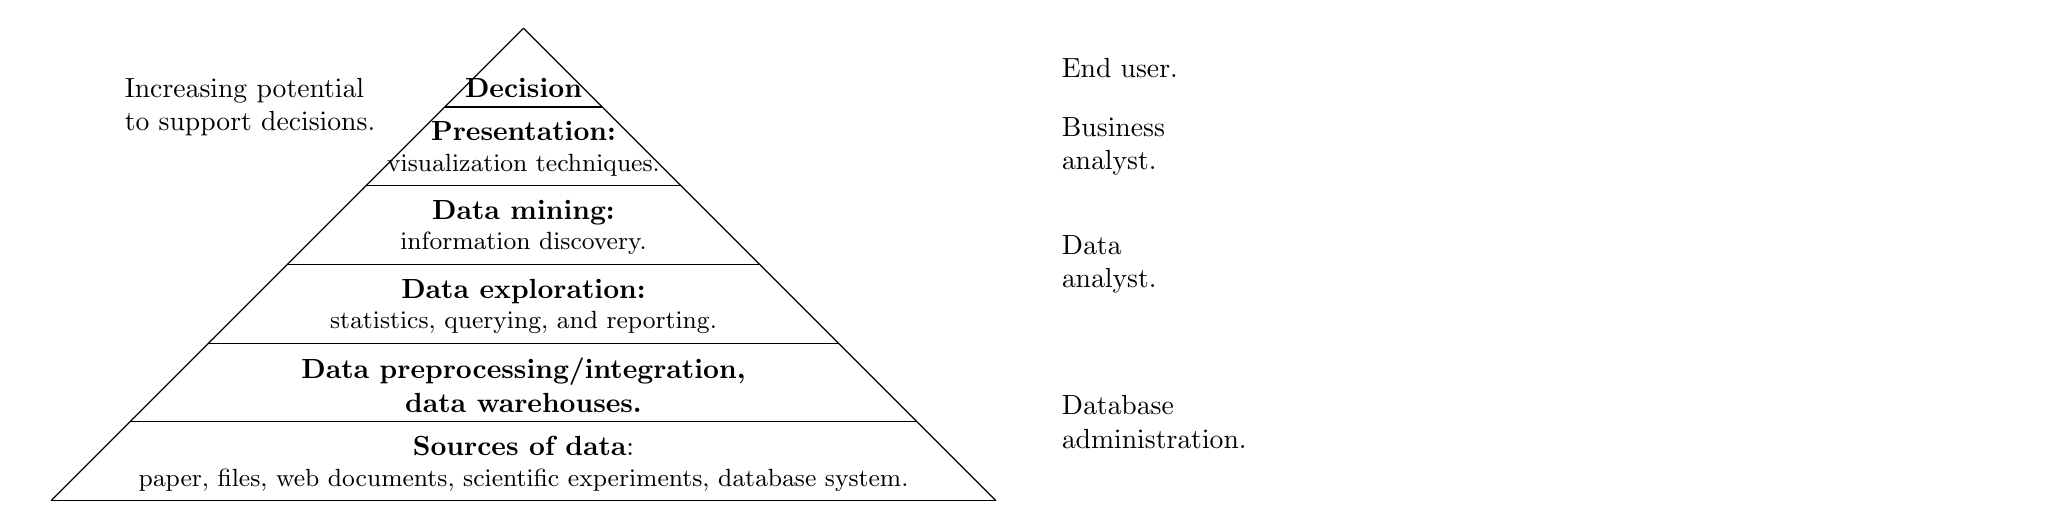
\begin{tikzpicture}
		\coordinate (A) at (-6,0) {};
		\coordinate (B) at ( 6,0) {};
		\coordinate (C) at (0,6) {};
		\draw[name path=AC] (A) -- (C);
		\draw[name path=BC] (B) -- (C);

		\node (Data Integration) at (1,5) {\parbox{\linewidth}{Increasing
				potential \\ to support decisions.}};
		\node (Data Integration) at (12.9,1) {\parbox{\linewidth}{Database \\
				administration.}};
		\node (Data Integration) at (12.9,3) {\parbox{\linewidth}{Data \\
				analyst.}};
		\node (Data Integration) at (12.9,4.5) {\parbox{\linewidth}{Business \\
				analyst.}};
		\node (Data Integration) at (12.9,5.5) {\parbox{\linewidth}{End user.}};

		\foreach \y/\A in {
		0/{
		\parbox{\linewidth}{
			\centering
			\textbf{Sources of data}: \\
			\small{paper, files, web documents, scientific experiments,
				database system.}}
		},
		1/{
		\parbox{\linewidth}{
			\centering
			\textbf{Data preprocessing/integration,\\
				data warehouses.}}
		},
		2/{
		\parbox{\linewidth}{
			\centering
			\textbf{Data exploration:} \\
			\small{statistics, querying, and reporting.}}
		},
		3/{
		\parbox{\linewidth}{
			\centering
			\textbf{Data mining:} \\
			\small{information discovery.}}
		},
		4/{
		\parbox{\linewidth}{
			\centering
			\textbf{Presentation:} \\
			\small{visualization techniques.}}
		},
		5/{
		\parbox{\linewidth}{
			\centering
			\textbf{Decision}}
		}
		} {
		\path[name path=horiz] (A|-0,\y) -- (B|-0,\y);
		\draw[name intersections={of=AC and horiz,by=P},
			name intersections={of=BC and horiz,by=Q}] (P) -- (Q)
		node[midway,above] {\A};
		}
	\end{tikzpicture}
\end{frame}

\begin{frame}{Data Mining in the Machine Learning and Statistics Community}
	Machine-learning and statistics communities usually classify data mining as
	the central part of their pipeline:

	\vspace{0.5cm}
	\centering
	\scalebox{0.95}{%
		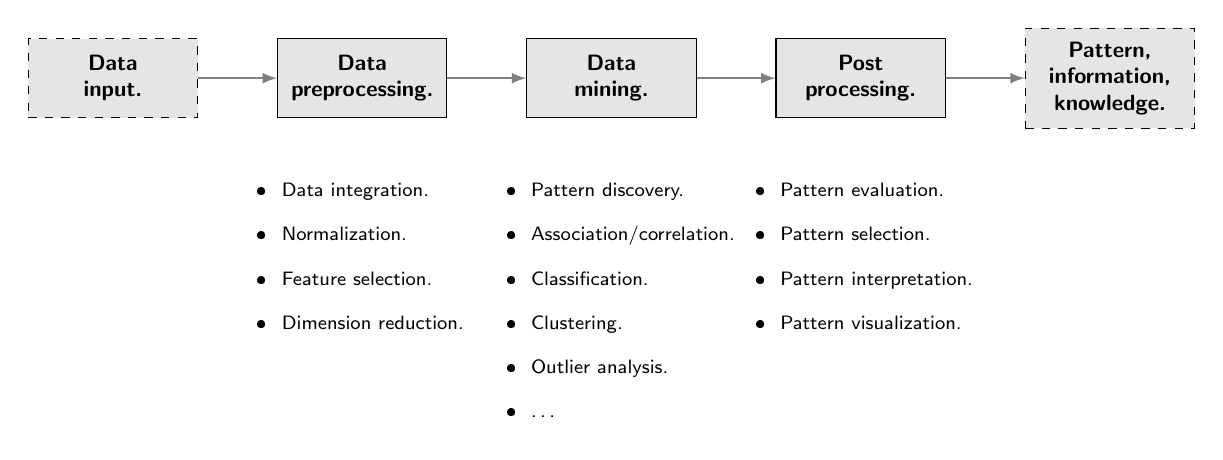
\begin{tikzpicture}
			[node distance = 1cm, auto,font=\footnotesize,
				% STYLES
				every node/.style={node distance=1cm},
				% The comment style is used to describe the characteristics of each
				%force
				comment/.style={rectangle, inner sep= 5pt, text width=3.8cm, node
						distance=0.5cm, font=\scriptsize\sffamily},
				% The force style is used to draw the forces' name
				force/.style={rectangle, draw, fill=black!10, inner sep=5pt, text
						width=1.8cm, text badly centered, minimum height=1cm,
						font=\bfseries\footnotesize\sffamily}]

			% Draw forces
			\node [force, dashed] (a) {\parbox{\linewidth}{\centering Data \\
					input.}};
			\node [force, right=1cm of a] (b) {\parbox{\linewidth}{\centering
					Data
					\\ preprocessing.}};
			\node [force, right=1cm of b] (c) {\parbox{\linewidth}{\centering
					Data
					\\ mining.}};
			\node [force, right=1cm of c] (d) {\parbox{\linewidth}{\centering
					Post
					\\ processing.}};
			\node [force, dashed, right=1cm of d] (e)
			{\parbox{\linewidth}{\centering Pattern, \\ information, \\
					knowledge.}};

			%%%%%%%%%%%%%%%
			% Change data from here

			% SUPPLIERS
			\node [comment, below=0.25cm of b] {
				\begin{itemize}
					\item Data integration.
					\item Normalization.
					\item Feature selection.
					\item Dimension reduction.
				\end{itemize}
			};

			% USERS
			\node [comment, below=0.25 of c] {
				\begin{itemize}
					\item Pattern discovery.
					\item Association/correlation.
					\item Classification.
					\item Clustering.
					\item Outlier analysis.
					\item \ldots
				\end{itemize}
			};

			% PUBLIC POLICIES
			\node [comment, below=0.25 of d] {
				\begin{itemize}
					\item Pattern evaluation.
					\item Pattern selection.
					\item Pattern interpretation.
					\item Pattern visualization.
				\end{itemize}
			};

			\path[->,thick]
			(a) edge (b)
			(b) edge (c)
			(c) edge (d)
			(d) edge (e);

		\end{tikzpicture}
	}
\end{frame}

\begin{frame}{The Data Mining Process: CRISP-DM}
	\begin{itemize}
		\item \textbf{CRoss-Industry Standard Process for Data Mining}:
	\end{itemize}
	\vspace{0.5cm}
	\centering
	\scalebox{0.95}{%
		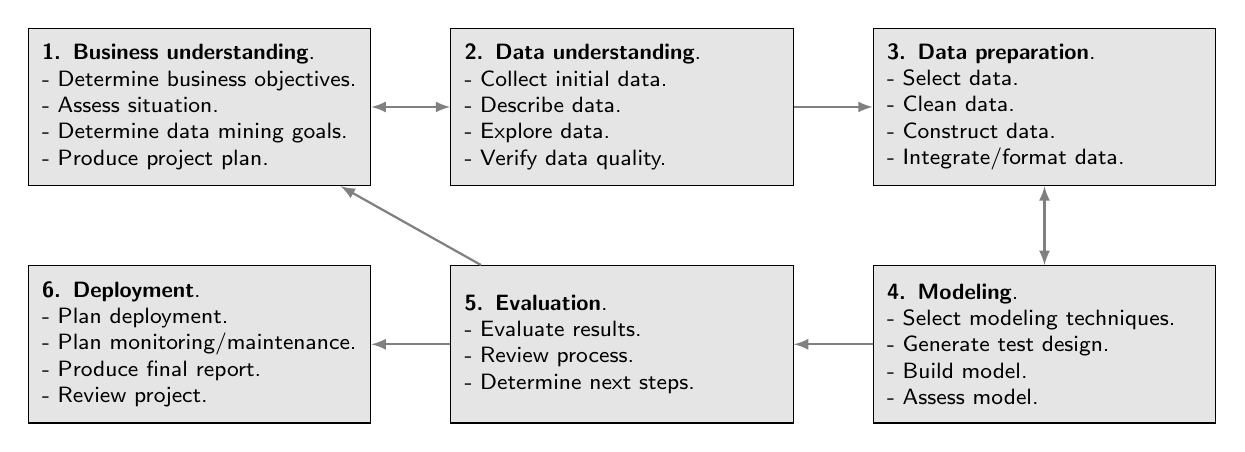
\begin{tikzpicture}
			[node distance = 2cm, auto,font=\footnotesize,
				% STYLES
				every node/.style={node distance=2cm},
				% The comment style is used to describe the characteristics of each
				%force
				comment/.style={rectangle, inner sep= 5pt, text width=5cm, node
						distance=0.5cm, font=\scriptsize\sffamily},
				% The force style is used to draw the forces' name
				force/.style={rectangle, draw, fill=black!10, inner sep=5pt, text
						width=4cm, minimum height=2cm, font=\footnotesize\sffamily}]

			% Draw forces
			\node [force] (a) {
				\parbox{\linewidth}{
					\textbf{1. Business understanding}.\\
					- Determine business objectives.\\
					- Assess situation.\\
					- Determine data mining goals.\\
					- Produce project plan.
				}
			};
			\node [force, right=1cm of a] (b) {
				\parbox{\linewidth}{
					\textbf{2. Data understanding}.\\
					- Collect initial data.\\
					- Describe data.\\
					- Explore data.\\
					- Verify data quality.
				}
			};
			\node [force, right=1cm of b] (c) {
				\parbox{\linewidth}{
					\textbf{3. Data preparation}.\\
					- Select data.\\
					- Clean data.\\
					- Construct data.\\
					- Integrate/format data.
				}
			};
			\node [force, below=1cm of c] (d) {
				\parbox{\linewidth}{
					\textbf{4. Modeling}.\\
					- Select modeling techniques.\\
					- Generate test design.\\
					- Build model.\\
					- Assess model.
				}
			};
			\node [force, below=1cm of a] (e) {
				\parbox{\linewidth}{
					\textbf{6. Deployment}.\\
					- Plan deployment.\\
					- Plan monitoring/maintenance.\\
					- Produce final report.\\
					- Review project.
				}
			};
			\node [force, below=1cm of b] (f) {
				\parbox{\linewidth}{
					\textbf{5. Evaluation}.\\
					- Evaluate results.\\
					- Review process.\\
					- Determine next steps.
				}
			};

			\path[->,thick]
			(b) edge (c)
			(d) edge (f)
			(f) edge (e)
			(f) edge (a);

			\path[<->,thick]
			(a) edge (b)
			(c) edge (d);
		\end{tikzpicture}
	}
\end{frame}

\section{A Multidimensional View of Data-Mining}

\begin{frame}{A Multidimensional View of Data Mining}
	\textbf{Data mining projects can be described in four dimensions:}
	\begin{itemize}
		\item \textbf{What data is available?}:\\
		      \small{
			      Data can exist in a wide variety of forms and must therefore be
			      treated differently in data mining.
		      }
		\item \textbf{What patterns are searched for?}:\\
		      \small{
			      Various functions in data mining can be used to detect
			      different patterns.
		      }
		\item \textbf{What technologies are used?}:\\
		      \small{
			      The technologies used can vary greatly in data mining.
		      }
		\item \textbf{What is the actual target application?}:\\
		      \small{
			      The actual target application also differs from case to case.
		      }
	\end{itemize}
\end{frame}

\section{What kind of data can be mined?}

\begin{frame}{What kind of data can be mined? (I)}
	\begin{itemize}
		\item \textbf{Any kind of data as long as meaningful for the target
			      application}
		\item Most basic forms of data sources:
		      \begin{itemize}
			      \item \textbf{Relational database:} \\
			            \small{Collection of tables, where the tables consist of a
				            set of attributes and usually a large set of tuples.}
			      \item \textbf{Data warehouse:} \\
			            \small{Repository of information collected from multiple
				            sources, stored under a unified schema.}
			      \item \textbf{Transactional database:} \\
			            \small{Captures transactions, such as customer purchases,
				            flight bookings, or user clicks on a website.}
		      \end{itemize}
	\end{itemize}
\end{frame}
\begin{frame}{What kind of data can be mined? (II)}
	\begin{itemize}
		\item Advanced data sets and advanced applications:
		      \begin{itemize}
			      \item Data streams and sensor data.
			      \item Time series data, temporal data, sequence data (incl.
			            biosequences).
			      \item Structure data, graphs, social networks and multi-linked data.
			      \item Object-relational databases.
			      \item Heterogeneous databases and legacy databases.
			      \item NoSQL databases.
			      \item Spatial data and spatiotemporal data.
			      \item Multimedia databases.
			      \item Text databases.
			      \item The world wide web.
		      \end{itemize}
	\end{itemize}
\end{frame}

\section{What kind of patterns can be mined?}

\begin{frame}{What kind of patterns can be mined?}
	\begin{itemize}
		\item \textbf{Searching for the right patterns is important.}
		\item Which patterns can be mined depends on:
		      \begin{itemize}
			      \item \textbf{Data mining function.} \\
			            \small{Different functions can reveal different patterns.}
			      \item \textbf{Data set.} \\
			            \small{Some types of records contain special patterns that
				            can be found only in them.}
		      \end{itemize}
		\item Patterns do not always lead to useful information. \\
		      $\rightarrow$ Always validate whether the gained knowledge is
		      interesting.
	\end{itemize}
\end{frame}

\begin{frame}{Data Mining Function: I. Generalization}
	\textbf{Information integration and data warehouse construction:}
	\begin{itemize}
		\item Data cleaning.
		\item Transformation.
		\item Integration.
		\item Multidimensional modeling.
	\end{itemize}
	\textbf{Data cube technology:}
	\begin{itemize}
		\item Characterization (contrast data characteristics).\\
		      E.g. dry vs. wet regions from numerical humidity values.
		\item Discrimination.
		\item Generalization.
		\item Summarization/Aggregation.
	\end{itemize}
\end{frame}

\begin{frame}{Data Mining Function: II. Association and Correlation Analysis}
	\textbf{Frequent patterns or item sets:}\\
	What items are frequently purchased together in your supermarket.\\[0.5cm]

	\textbf{Association, correlation vs. causality:}\\
	A typical association rule: Diapers $\rightarrow$ Beer $[0.5\%,75\%]$
	(support, confidence).\\
	Are strongly associated items also strongly correlated?\\[0.5cm]

	\textbf{How to mine such patterns and rules efficiently in large
		datasets?}\\
	\textbf{How to use such patterns for classification, clustering and other
		applications?}
\end{frame}

\begin{frame}{Data Mining Function: III. Classification}
	\textbf{Classification and (class-)label prediction:}\\
	Construct models (functions) based on training examples. \\
	Hence: "supervised".\\
	Describe and distinguish classes or concepts for future prediction.\\
	E.g. classify countries based on climate or classify cars based on gas
	mileage.\\
	Classifying something means to predict unknown class labels. \\[0.5cm]

	\textbf{Typical methods:}\\
	Decision trees, naive Bayesian classification, support-vector machines,
	neural networks, rule-based classification, pattern-based classification,
	logistic regression \ldots\\[0.5cm]

	\textbf{Typical applications:}\\
	Credit-card-fraud detection, direct marketing, classifying stars, diseases,
	web pages \ldots
\end{frame}

\begin{frame}{Data Mining Function: IV. Cluster Analysis}
	\textbf{Unsupervised learning:} I.e. class labels are unknown.\\
	\textbf{Group data:} I.e. cluster houses to find distribution
	patterns.\\[0.5cm]

	Principle:\\
	Maximize intra class similarity and minimize inter class
	similarity.\\[0.5cm]

	What is \textbf{similarity?}
\end{frame}

\begin{frame}{Data Mining Function: V. Outlier Analysis}
	\textbf{Outlier}: A data object that does not comply with the general
	behavior of the data.\\[0.5cm]

	Noise or exception?\\
	One person's garbage could be another person's treasure.\\[0.5cm]

	\textbf{Methods:}\\
	By-product of clustering or regression analysis. \\
	Useful in fraud detection or rare-events analysis.
\end{frame}

\begin{frame}{Time and Ordering: VI. Sequential Pattern, Trend and Evolution
		Analysis}
	\textbf{Sequence, trend, and evolution analysis}.\\
	\begin{itemize}
		\item Trend, time-series, and deviation analysis. \\
		      E.g., regression and value prediction (forecasting).
		\item Sequential-pattern mining.\\
		      E.g. customers first buy a digital camera, then buy large SD memory
		      cards.
		\item Periodicity analysis.
		\item Motifs and biological-sequence analysis.\\
		      Approximate and consecutive motifs.
		\item Similarity-based analysis.\\
		\item Mining data streams.\\
		      Ordered, time-varying, potentially infinite (unbounded).
	\end{itemize}
\end{frame}

\begin{frame}{Structure and Network Analysis}
	\textbf{Graph mining}:\\
	Finding frequent subgraphs (e.g. chemical compounds), trees (XML),
	substructures (web fragments), information-network analysis.\\[0.2cm]

	\textbf{Social networks}:
	\begin{itemize}
		\item Social networks: Actors (objects, nodes) and relationships
		      (edges).\\
		      E.g., author networks in CS, terrorist networks.
		\item Multiple heterogeneous networks.\\
		      A person could be in multiple information networks such as friends, family,
		      classmates.
		\item Links carry a lot of semantical information: link mining.
	\end{itemize}

	\textbf{Web mining}:
	\begin{itemize}
		\item Web is a big information network: from PageRank to Google.
		\item Analysis of web information networks.
		\item Web community discovery, opinion mining, usage mining.
	\end{itemize}
\end{frame}

\begin{frame}{Evaluation of Knowledge}
	\textbf{Is all mined knowledge interesting?}
	\begin{itemize}
		\item One can mine tremendous amounts of "patterns" and knowledge.
		\item Some may fit only certain dimension space (e.g. time, location).
		\item Some may not be representative, may be transient.
	\end{itemize}

	\textbf{Evaluation of mined knowledge $\rightarrow$ directly mine only
		interesting knowledge?}
	\begin{itemize}
		\item Descriptive vs. predictive.
		\item Coverage.
		\item Typically vs. predictive.
		\item Accuracy.
		\item Timeliness.
		\item \ldots
	\end{itemize}
\end{frame}

\section{What technologies are used?}

\begin{frame}{Data Mining: Confluence of Multiple Disciplines}
	\centering
	\resizebox{5.5cm}{5.5cm}{%
		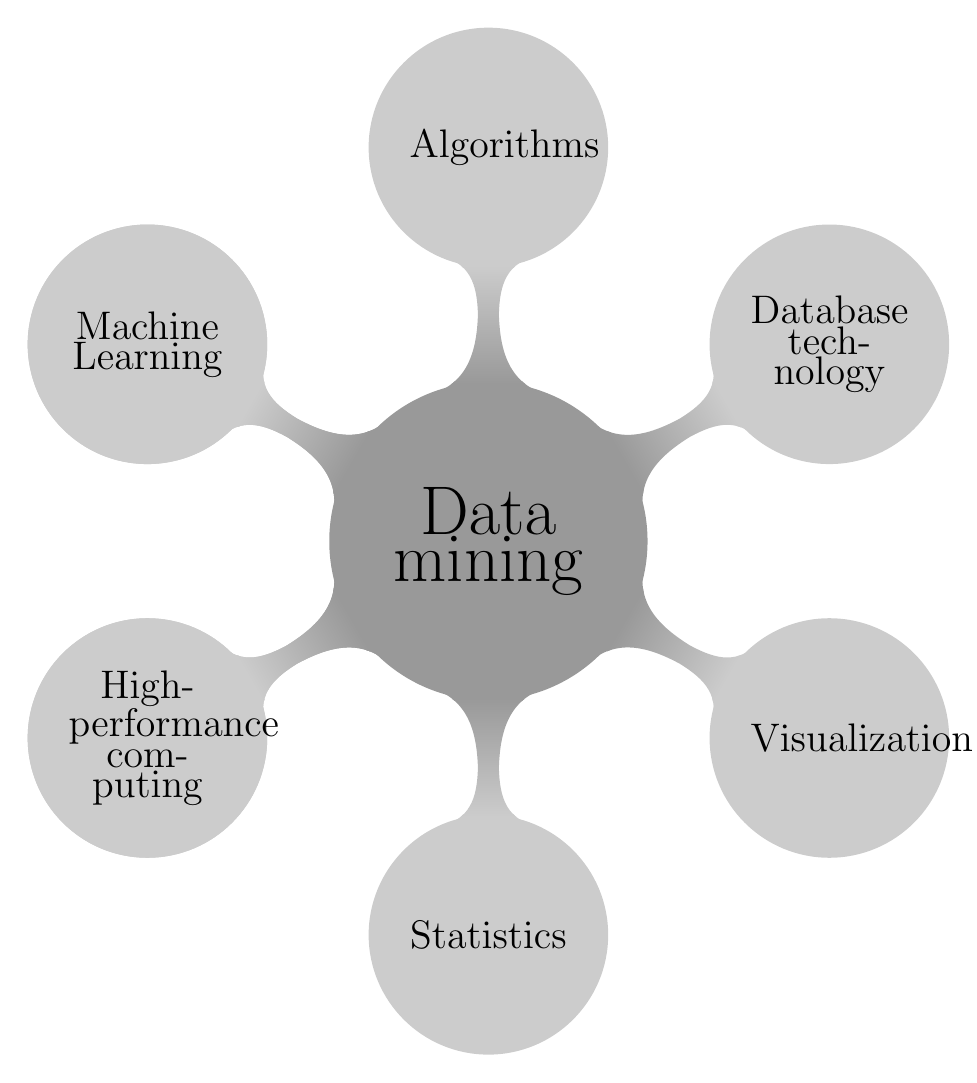
\begin{tikzpicture}[mindmap, minimum size=4cm, every
				node/.style=concept, concept color=black!40, grow cyclic]
			\node[concept] {\Huge Data mining}
			child [concept color=gray!40, minimum size=3cm]{node {\Large
							Machine Learning}}
			child [concept color=gray!40, minimum size=3cm]{node {\Large
							Pattern recognition}}
			child [concept color=gray!40, minimum size=3cm]{node {\Large
							Statistics}}
			child [concept color=gray!40, minimum size=3cm]{node {\Large
							Visualization}}
			child [concept color=gray!40, minimum size=3cm]{node {\Large
							Database technology}}
			child [concept color=gray!40, minimum size=3cm]{node {\Large
							Algorithms}}
			child [concept color=gray!40, minimum size=3cm]{node {\Large
							Machine Learning}}
			child [concept color=gray!40, minimum size=3cm]{node {\Large
							High-performance computing}};
		\end{tikzpicture}}
\end{frame}

\begin{frame}{Why Confluence of Multiple Disciplines?}
	\textbf{Tremendous amount of data:}
	\begin{itemize}
		\item Algorithms must be highly scalable to handle also terabytes of
		      data.
	\end{itemize}

	\textbf{High dimensionality of data:}
	\begin{itemize}
		\item DNA microarrays may have tens of thousands of dimensions.\\
		      Collections of microscopic DNA spots attached to a solid surface.
	\end{itemize}

	\textbf{High complexity of data:}
	\begin{itemize}
		\item Data streams and sensor data.
		\item Time-series data, temporal data, sequence data.
		\item Structure data, graphs, social networks, and multi-linked data.
		\item Heterogeneous databases and legacy databases.
		\item Spatial, spatiotemporal, multimedia, text and web data.
		\item Software programs, scientific simulations.
	\end{itemize}
	\textbf{New and sophisticated applications.}
\end{frame}

\section{What kind of applications are targeted?}

\begin{frame}{Applications of Data Mining (I)}
	\begin{itemize}
		\item \textbf{Wherever there is data and more knowledge is desired,
			      there are data mining applications.}\\
		\item Typical data mining applications:
		      \begin{itemize}
			      \item \textbf{Business Intelligence} \\
			            \small{Provides historical, current, and predictive views of
				            business operation.}
			      \item \textbf{Web Search Engines} \\
			            \small{Need to decide which pages to index, which ones to
				            index and how to rank them for search.}
			      \item \textbf{Fraud detection} \\
			            \small{Possible fraud attempts automatically based on
				            suspicious patterns in transactions.}
			      \item \textbf{Predictive Maintenance} \\
			            \small{Evaluation of sensor data to maintain machines in time
				            before a defect occurs.}
		      \end{itemize}
	\end{itemize}
\end{frame}

\begin{frame}{Applications of Data Mining (II)}
	\begin{itemize}
		\item Example research projects using data mining at FAU\footnote{Found
			      in the FAU CRIS (Current research information system):
			      \url{https://cris.fau.de/}}:
		      \begin{itemize}
			      \item \textbf{Prediction of product properties using data mining
				            methods.} \\
			            \small{Prof. Dr.-Ing. Sandro Wartzack (Chair of Engineering
				            Design)}
			      \item \textbf{Combustion and fuel optimization for the utilization
				            of residues in biomass furnaces.} \\
			            \small{Prof. Dr.-Ing. Jürgen Karl (Chair of Energy Process
				            Engineering)}
			      \item \textbf{CoralTrace – A new approach to understanding
				            climate-induced reef crises.} \\
			            \small{Prof. Dr. Wolfgang Kießling (Chair of Palaeontology)}
			      \item \textbf{Performance Analysis in Team Sports.} \\
			            \small{Prof. Dr. Björn Eskofier (Machine Learning and Data
				            Analytics Lab)}
			      \item \textbf{And many more.} \\
			            \small{Chair of computer science 6 (data management)
				            has some projects related to data mining, too. More
				            information will be given in the last lecture.}
		      \end{itemize}
	\end{itemize}
\end{frame}

\section{Major issues in data mining}

\begin{frame}{Major Issues in Data Mining (I)}
	\textbf{Mining methodology:}\\
	\begin{itemize}
		\item Mining various and new kinds of knowledge.
		\item Mining knowledge in multi-dimensional space.
		\item Data mining: An interdisciplinary effort.
		\item Boosting the power of discovery in a networked environment.
		\item Handling noise, uncertainty, and incompleteness of data.
		\item Pattern evaluation and pattern- or constraint-guided mining.
	\end{itemize}
	\textbf{User interaction:}\\
	\begin{itemize}
		\item Interactive mining.
		\item Incorporation of background knowledge.
		\item Presentation and visualization of data mining results.
	\end{itemize}
\end{frame}

\begin{frame}{Major Issues in Data Mining (II)}
	\textbf{Efficiency and scalability:}\\
	\begin{itemize}
		\item Efficiency and scalability of data-mining algorithms.
		\item Parallel, distributed, stream and incremental mining methods.
	\end{itemize}
	\textbf{Diversity of data types:}\\
	\begin{itemize}
		\item Handling complex types of data.
		\item Mining dynamic, networked and global data repositories.
	\end{itemize}
	\textbf{Data mining and society:}\\
	\begin{itemize}
		\item Social impacts of data mining.
		\item Privacy-preserving data mining.
		\item Invisible data mining.
	\end{itemize}
\end{frame}

\section{Summary}

\begin{frame}{Summary}
	\textbf{Data mining:}\\
	Discovering interesting patterns and knowledge from massive amounts of
	data.\\[0.2cm]

	\textbf{A natural evolution of database technology:}\\
	In great demand, with wide applications.\\[0.2cm]

	\textbf{KDD pipeline includes:}\\
	Data cleaning, data integration, data selection, transformation, data
	mining, pattern evaluation and knowledge presentation.\\[0.2cm]

	\textbf{Mining can be performed in a variety of data.}\\
	\textbf{Data-mining functionalities:}\\
	Characterization, discrimination, association, classification, clustering,
	outlier and trend analysis, etc.\\[0.2cm]

	\textbf{Data-mining technologies and applications.}\\
	\textbf{Major issues in data mining.}\\
\end{frame}

\begin{frame}[c]
	\begin{center}
		{\bf Any questions about this chapter?}\\[0.5cm]
		Ask them now or ask them later in our forum: \\\bigskip
		\qrcode{https://www.studon.fau.de/studon/goto.php?target=lcode_OLYeD79h} \\
		\vspace*{0.5cm}
		\faLink\ \url{https://www.studon.fau.de/studon/goto.php?target=lcode_OLYeD79h} \smallskip

	\end{center}
\end{frame}

\section*{Appendix}

\begin{frame}{Further Improvements of Mining Methods}
	\begin{itemize}
		\item \textbf{AFOPT} (Liu et al., KDD'03)
		      \begin{itemize}
			      \item A "push-right" method for mining condensed frequent-pattern
			            (CFP) tree.
		      \end{itemize}
		\item \textbf{Carpenter} (Pan et al., KDD'03)
		      \begin{itemize}
			      \item Mine datasets with small rows but numerous columns.
			      \item Construct a row-enumeration tree for efficient mining.
		      \end{itemize}
		\item \textbf{FP-growth+} (Grahne \& Zhu, FIMI'03)
		      \begin{itemize}
			      \item Efficiently using prefix-trees in mining frequent itemsets.
		      \end{itemize}
		\item \textbf{TD-Close} (Liu et al., SDM'06)
	\end{itemize}
\end{frame}

\begin{frame}{Extension of Pattern-growth Mining Methodology}
	\begin{itemize}
		\item \textbf{Mining closed frequent itemsets and max-patterns.}
		      \begin{itemize}
			      \item CLOSET (DMKD'00), FPclose, and FPMax (Grahne \& Zhu, FIMI'03)
		      \end{itemize}
		\item \textbf{Mining sequential patterns.}
		      \begin{itemize}
			      \item PrefixSpan (ICDE'01), CloSpan (SDM'03), BIDE (ICDE'04)
		      \end{itemize}
		\item \textbf{Mining graph patterns.}
		      \begin{itemize}
			      \item gSpan (ICDM'02), CloseGraph (KDD'03)
		      \end{itemize}
		\item \textbf{Constraint-based mining of frequent patterns.}
		      \begin{itemize}
			      \item Convertible constraints (ICDE'01), gPrune (PAKDD'03)
		      \end{itemize}
		\item \textbf{Computing iceberg data cubes with complex measures.}
		      \begin{itemize}
			      \item H-tree, H-cubing, and Star-cubing (SIGMOD'01, VLDB'03)
		      \end{itemize}
		\item \textbf{Pattern-growth-based clustering.}
		      \begin{itemize}
			      \item MaPle (Pei et al., ICDM'03)
		      \end{itemize}
		\item \textbf{Pattern-growth-based classification.}
		      \begin{itemize}
			      \item Mining frequent and discriminative patterns (Cheng et al.,
			            ICDE'07)
		      \end{itemize}
	\end{itemize}
\end{frame}

\begin{frame}{Visualization of Association Rules (I)}
	\centering
	\scalebox{0.9}{
		\includegraphics[width=0.6\textwidth]{img/assoc_rules1.jpg}
	}
	% In fact, these two illustrations are still the best visualization of association rules I could find. Alternatives would % be the visualizations from e.g. this Jupyter Notebook experiment:
	% https://goldinlocks.github.io/Market-Basket-Analysis-in-Python/.
	% It may also be useful to revisit these graphics once we have completed our exercise sheets.
\end{frame}

\begin{frame}{Visualization of Association Rules (II)}
	\centering
	\scalebox{0.9}{
		\includegraphics[width=0.6\textwidth]{img/assoc_rules2.jpg}
	}
\end{frame}


\end{document}
